\chapter*{Números Reales}
\setcounter{chapter}{1}
\section{Conjuntos}
$$\N = \{1,2,3,4,5,\dots\}$$
$$\N^0 = \{0,1,2,3,4,5,\dots\}$$

$$\Z = \{\dots,-3,-2,-1,0,1,2,3,\dots\}$$
$$\Z^+ = \{1,2,3,4,5,\dots\}$$
$$\Z^- = \{\dots,-5,-4,-3,-2,-1\}$$

\myparagraph{\underline{Divisibilidad:}}
$a$ es divisible por $b$ si hay un entero $k$ tal que:
{\large$$a = b \cdot k $$}

\begin{paragraph}
    {\underline{Conjuntos de números enteros}}
    \begin{itemize}
        \item {\textbf{Números pares:} $\{2k: k \in \Z\}$}
        \item {\textbf{Números impares:} $\{2k +1 : k \in \Z\}$}
        \item {\textbf{Números primos:} $p$ es primo si tiene sólo 2    divisores: $1$ y $p$}
        \item {\textbf{Números compuestos:} Números que no son primos}
        \item[*]{1 no es ni primo ni compuesto}
    \end{itemize}
\end{paragraph}

\yellowBox{Teoría fundamental de la artitmética}{
    Todo número natural $n$ mayor que 1 tiene una única factorización en números primos.
    \tcblower
    \begin{center}
        \textbf{Ejemplo:}
        \begin{itemize}
            \item {$n = 120 \Rightarrow 2 \cdot 2 \cdot 2 \cdot 3 \cdot 5 \Rightarrow 2^3 \cdot 3 \cdot 5$}
            \item {$n = 15 \Rightarrow 15 = 3 \cdot 5$}
        \end{itemize}
    \end{center}
}

\yellowBox{Máximo común divisor - MCD}{
    $a$, $b$ y $d$ son números entreros. Si $d|a$ y $d|b$ se dice que $d$ es un Divisor común de $a$ y $b$. El mayor de estos divisores comunes es el \textbf{máximo común divisor}

    *Si el MCD de dos enteros es 1, $a$ y $b$ son \textbf{coprimos}
    \tcblower
    \begin{center}
        \textbf{Ejemplo:}\\
    \end{center}
        $a = 15, b = 8 \Rightarrow MCD(a,b) = 1 \rightarrow \text{a y b son \textbf{coprimos}}$
}

\section{Recta Numérica}
\begin{center}
    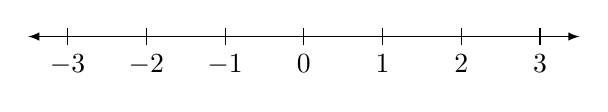
\begin{tikzpicture}
    \draw[latex-latex] (-3.5,0) -- (3.5,0) ; %edit here for the axis
    \foreach \x in  {-3,-2,-1,0,1,2,3} % edit here for the vertical lines
    \draw[shift={(\x,0)},color=black] (0pt,3pt) -- (0pt,-3pt);
    \foreach \x in {-3,-2,-1,0,1,2,3} % edit here for the numbers
    \draw[shift={(\x,0)},color=black] (0pt,0pt) -- (0pt,-3pt) node[below] 
    {$\x$};
    \end{tikzpicture}
\end{center}

\section{Conjunto Racional}
\yellowBox{Definición - Conjunto Racional}{
    \[\Q \rightarrow \text{Conjunto de todas las fracciones } \frac{a}{b} \text{ donde } a \text{, } b \in \Z \text{ y } b \neq 0 \text{.}\]
    \[\Q = \left\{ \frac{a}{b} : a \in \Z, b \in \Z - \{0\} \right\} \]

}

\begin{center}
    \Large{
        $\text{M} 
        \in 
        \N 
        \Rightarrow 
        \frac{a}{b}$ = $\frac{a \cdot M}{b \cdot M}$
    }
\end{center}

\blueBox{Fracciones equivalentes}{
    \[\frac{a}{b} = \frac{c}{d} \text{ si y solo si } a \cdot d = b \cdot c \]
}

\paragraph{Operaciones con racionales}
\begin{itemize}
    % \textbf{Suma: \Rightarrow } $\frac{a}{b} \text{+} \frac{c}{b} \text{=} \frac{a+c}{b}$
    \item {\textbf{Suma: } \Large{$\frac{a}{b} + \frac{c}{b} = \frac{a+c}{b}$}}
    \item {\textbf{Multiplicación: } \Large{$\frac{a}{b} \cdot \frac{c}{d} = \frac{a \cdot c}{b \cdot d}$}}
    \item {\textbf{División: } \Large{$\frac{a}{b} : \frac{c}{d} = \frac{a}{b} \cdot \frac{d}{c} = \frac{a \cdot d}{b \cdot c}$}}
        
\end{itemize}

\section{Representación de los racionales en la recta}
\yellowBox{Teorema de Thales}{
    Dos rectas cortadas por rectas paralelas $\rightarrow$ los segmentos cortados son proporcionales.
}

\begin{center}
    \includegraphics[width=0.5\linewidth]{thales.jpg}
    $$\frac{AB}{A'B'} = \frac{BC}{B'C'} = \frac{CD}{C'D'}$$
\end{center}

\yellowBox{Definición - Orden en $\Q$}{
    Sean {\large$\frac{a}{b}$} y {\large$\frac{c}{d}$} dos fracciones con $b$ y $d$ positivos $\Rightarrow$ {\large$\frac{a}{b} < \frac{c}{d}$} si y solo si 
    $$a \cdot d < b \cdot c$$
    Igualmente, dadas {\large$\frac{a}{b}$} y {\large$\frac{c}{d}$} dos fracciones con $b$ y $d$ positivos $\Rightarrow$ {\large$\frac{a}{b}$} $\leq$ {\large$\frac{c}{d}$} si
    $$a \cdot d \leq b \cdot c$$
    \tcblower
    \begin{center}
        \textbf{Ejemplo:}\\
        $$\frac{1}{3} < \frac{\frac{1}{3} + \frac{1}{2}}{2} < \frac{1}{2} \text{ es decir, } \frac{1}{3} < \frac{5}{12} < \frac{1}{2}$$
    \end{center}
}

\blueBox{Propiedad}{
    Entre dos racionales distintos en la recta numérica, extisten infinitos puntos que representan números racionales.
}

\section{Reresentación decimal de los racionales}
Páginas 8 - 13

\section{Números Reales}
Dados dos conjuntos $A$ y $B$, se llama $\emph{unión}$ de $A$ y $B$ al conjunto de todos los elementos que están en el conjunto $A$ o en el conjunto $B$.

$$A \cup B = \{x: x \in A \vee x \in B\}$$
\begin{center}
    $x$ pertenece a $A$ o $x$ pertenece a $B$
\end{center}

$$A \cap B = \{x: x \in A \wedge x \in B\}$$
\begin{center}
    $x$ pertenece a $A$ y $x$ pertenece a $B$
\end{center}

\blueBox{Número Reales}{
    El conjunto de los reales es la unión de los números racionales y los números irracionales.
    $$\R = \Q \cup \mathbb{I}$$
    Por lo tanto, el conjunto de los números reales está formado por todos los números que admiten una representación decimal, finita o infinita y tanto periódica como no periódica.
}

\paragraph{Propiedades de la suma:}
\begin{enumerate}
    \item (Asociatividad): $\forall \: a, b, c \in \R \Rightarrow a + (b + c) = (a + b) + c$
    \item (Comutatividad): $\forall \: a, b \in \R \Rightarrow a + b = b + a$
    \item (Existencia del elemento neutro) $\exists \: 0 \in \R \text{ tal que } \forall \: a \in \R \Rightarrow a + 0 = a$
    \item (Existencia de opuestos) $\forall \: a \in \R \: \exists \: -a \in \R \text{ tal que } a + (-a) = 0$   
\end{enumerate}

\paragraph{Propiedades de la multiplicación:}
\begin{enumerate}
    \item (Asociatividad): $\forall \: a, b, c \in \R \Rightarrow a \cdot (b \cdot c) = (a \cdot b) \cdot c$
    \item (Comutatividad): $\forall \: a, b \in \R \Rightarrow a \cdot b = b \cdot a$
    \item (Existencia del identidad) $\exists \: 1 \in \R \text{ tal que } \forall \: a \in \R \Rightarrow a \cdot 1 = a$
    \item (Existencia de inverso multiplicativo) $\forall \: a \in \R-\{0\} \; \exists \; a^{-1} \in \R \text{ tal que } a \cdot a^{-1} = 1$
\end{enumerate} 

\myparagraph{Propiedad distributiva de la multiplicación respecto de la suma:}
$\forall \: a, b, c \in \R$:
$$a \cdot (b+c) = a \cdot b + a \cdot c$$

\paragraph{Leyes cancelativas:}
\begin{itemize}
    \item[1.] $a+b = a+c \Rightarrow b = c$
    \item[2.] $a \cdot b = a \cdot c \Rightarrow b = c$
    \item $\emph{Restar}$ es sumar el opuesto, $a-b = a + (-b)$
    \item $\emph{Dividir}$ es multiplicar por el inverso, $a/b = a \cdot b^{-1} \: \text{con}\: b \neq 0$
\end{itemize} 

\section{Intervalos Reales.}
\paragraph{Intervalos acotados.}
\begin{itemize}
    \item $(a,b) = \{x \in \R : a < x < b\} \: \emph{Intervalo abierto}$
    \item $[a,b] = \{x \in \R : a \leq x \leq b\} \: \emph{Intervalo cerrado}$
    \item $[a,b) = \{x \in \R : a \leq x < b\} \: \emph{Intervalo semicerrado por izquieda}$
    \item $(a,b] = \{x \in \R : a < x \leq b\} \: \emph{Intervalo semicerrado por derecha}$
\end{itemize}

\paragraph{Intervalos no acotados.}
\begin{itemize}
    \item $(-\infty, a) = \{x \in \R : x < a\}$
    \item $[a, +\infty) = \{x \in \R : x \geq a\}$
    \item[*] $(-\infty, +\infty) = \R$
\end{itemize}

\section{Valor Absoluto}

\yellowBox{Definición - Valor Absoluto}{
    Dado un número real \emph{x} se llama \emph{valor absoluto} de \emph{x} al número real $|x|$ tal que:
    $$
    |x| = \begin{cases}
            \phantom{-}x & \text{si } x \geq 0 \\
            -x & \text{si } x < 0
    \end{cases}
    $$
    El valor absoluto o módulo de un número real, puede interpretarse como la distancia de dicho número al origen en la recta numérica.
}

\blueBox{Propiedades - valor absoluto}{
    Sean $a, b \in \R$ y $k > 0$:
    \begin{enumerate}
        \item $|a| \geq 0$
        \item $|a \cdot b| = |a| \cdot |b|$
        \item $|a| = |-a|$
        \item $|a| \leq k \; \text{equivale a} \; -k \leq a \; \leq k$
        \item $|a| \geq k \; \text{equivale a} \; a \leq -k \; \text{o bien} \; k \leq a$
        \item $|a+b| \leq |a| + |b|$ (desiguldad triangular)
    \end{enumerate}
}

\section{Exponentes y raíces}
\myparagraph{Potenciación}
Cualquier número real $a$ y cualquier número natural $n$ se define la potencia $a^n$ como el producto de $n$ copias de $a$:
{\large$$a^n = \underbrace{a \cdot a \: ... \: a}_{\text{n-veces}}$$}

\blueBox{Propiedades - Potenciación}{
    Dados $a, b \in \R$ y $n, m \in \N$:
    \begin{enumerate}
        \item {$a^m \cdot a^n = a^{m+n}$  (Producto de potencias de igual base)}
        \item {$\text{\Large $\frac{a^m}{a^n}$} = a^{m-n}$ (Cociente d epotencias de igual base ($a \neq 0$))} 
        \item {$(a^m)^n = a^{m \cdot n}$ (Potencia de potencia)}
        \item {$(a \cdot b)^n = a^n \cdot b^n$ (La potenciación es distributiva respecto de la multiplicación)}
        \item {$\text{\Large $\bigl(\frac{a}{b} \bigr)$}^n = \text{\Large $\frac{a^n}{b^n}$} \; \; b \neq 0$ (La potenciación es distributiva respecto de la división)}
    \end{enumerate}
}

\myparagraph{Radicación}
Dado un número real $a \geq 0$, el símbolo $\sqrt{a}$ denota al único número real no negativo que al elevarlo al cuadrado da como resultado $a$:
{\large $$\sqrt{a} = b \Leftrightarrow b^2 = a \; \text{y} \; b \geq 0$$}

\yellowBox{Definición - (raíz \emph{n}-ésima)}{
    {\large$$\sqrt[n]{a} = b \Leftrightarrow b^n = a$$}
    $n \in \Z > 1$. Si $n$ es par, entonces $a \geq 0$ y $b \geq 0$.
}

\blueBox{Propiedades - radicación}{
    \begin{enumerate}
        \item $\sqrt[n]{a \cdot b} = \sqrt[n]{a} \cdot \sqrt[n]{b}$ (a y b deben ser no negativos en el caso n par)
        \item $\text{\Large $\sqrt[n]{\frac{a}{b}}$} = \text{\Large $\frac{\sqrt[n]{a}}{\sqrt[n]{b}}$}$ (a y b deben ser no negativos en el caso n par, además b debe ser, en cualquier caso, distinto de 0)
        \item $\sqrt[n]{\sqrt[m]{a}} = \sqrt[n \cdot m]{a}$ (a debe ser no negativo si n o m fuesen pares)
    \end{enumerate} 
}

$$a^{\frac{m}{n}} = \sqrt[n]{m}$$

\myparagraph{\large Racionalización de denominadores}
Para hacer representaciones con fracciones que tienen denominadores irracionales suele ser dificil, por lo que hay que convertirlos en fracciones con denominadores racionales. Para ello se utiliza la siguiente técnica:\\

\textbf{Ejemplo 1.} Racionalizar {\Large $\frac{4}{\sqrt{3}}$}\\
\emph{Teniendo en cuenta que $\sqrt{3} \cdot \sqrt{3} = 3$ y que {\Large $\frac{\sqrt{3}}{\sqrt{3}} = 1$}, multiplicamos y divimos la fracción por $\sqrt{3}$:}
$$\frac{4}{\sqrt{3}} = \frac{4}{\sqrt{3}} \cdot \frac{\sqrt{3}}{\sqrt{3}} = \frac{4 \cdot \sqrt{3}}{3}$$

\textbf{Ejemplo 2.} Racionalizar {\Large $\frac{1}{\sqrt[3]{12}}$}

$$\frac{1}{\sqrt[3]{12}} = \frac{1}{\sqrt[3]{2^2 \cdot 3}} = \frac{1}{\sqrt[3]{2^2 \cdot 3}} \cdot \frac{\sqrt[3]{2 \cdot 3^2}}{\sqrt[3]{2 \cdot 3^2}} = \frac{\sqrt[3]{18}}{\sqrt[3]{2^3 \cdot 3^3}} = \frac{\sqrt[3]{18}}{6}$$

\textbf{Ejemplo 3.} Racionalizar {\Large $\frac{2}{\sqrt{5} + \sqrt{6}}$}
\begin{gather*}
{\frac{2}{\sqrt{5} + \sqrt{6}} = \frac{2}{\sqrt{5} + \sqrt{6}} \cdot \frac{\sqrt{5} - \sqrt{6}}{\sqrt{5} - \sqrt{6}} = \frac{2 \cdot (\sqrt{5} - \sqrt{6})}{(\sqrt{5})^2 - (\sqrt{6})^2}} \\ 
{= \frac{2 \cdot (\sqrt{5} - \sqrt{6})}{-1} = 2 \cdot (\sqrt{6} - \sqrt{5})}
\end{gather*}

\section{Elementos de la geometría}
\paragraph{Ángulos.}
\begin{itemize}
    \item{Complementarios: dos ángulos que suman 90º}
    \item{Suplementarios: dos ángulos que suman 180º}
\end{itemize}

\begin{center}
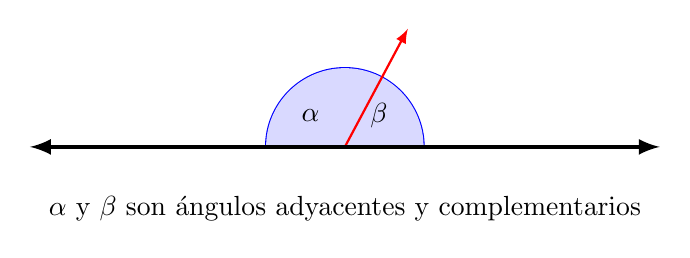
\begin{tikzpicture}
    % Draw a line that will be used as a reference for the angle with full arrows at both ends
    % draw semicirle with radius 1 on top of the line
    \draw[thick, blue] (1,0) arc (0:180:1);
    \fill[blue!15] (1,0) arc (0:180:1);
    % Draw a line from the center of the reference line at 60 degrees
    \draw[thick, red, -latex] (0,0) -- (0.8,1.5);
    \draw[ultra thick, latex-latex] (-4,0) -- (4,0);
    % write alpha and beta to the sides of the red line
    \node[above, right] at (0.2,0.4) {$\beta$};
    \node[above, left] at (-0.2,0.4) {$\alpha$};

    % add text below graphic to explain what is drawn
    \node[below] at (0,-0.5) {$\alpha$ y $\beta$ son ángulos adyacentes y complementarios};

\end{tikzpicture}
\end{center}

\myparagraph{Triángulos}
\textbf{Clasificación por lados:}
\begin{itemize}
    \item{Equilátero: tres lados iguales}
    \item{Isósceles: dos lados iguales}
    \item{Escaleno: tres lados distintos}
\end{itemize}
\textbf{Clasificación por ángulos:}
\begin{itemize}
    \item{Acutángulo: tres ángulos agudos}
    \item{Rectángulo: un ángulo recto}
    \item{Obtusángulo: un ángulo obtuso}
\end{itemize}

\blueBox{Propiedades}{
    \begin{enumerate}
        \item (Desigualdad triangular) La suma de los dos lados menores de un triángulo es mayor que el lado mayor.
        $$\overline{AB} + \overline{BC} > \overline{AC}$$
        \item En todo tríangulo, a mayor lado se opone mayor ángulo
    \end{enumerate}
}

\noindent
\textbf{\emph{\underline{Mediana:} }} Línea que une un vértice con el punto medio del lado opuesto.\\
\textbf{\emph{\underline{Mediatriz:} }} Línea que pasa por el medio del lado de forma perpendicular.\\
\textbf{\emph{\underline{Altura:} }} Línea perpendicular al lado opuesto al vértice que se toca.\\

$$\boxed{A = \frac{B \cdot h}{2}}$$
\begin{center}
    Fórmula del área de un triángulo, siendo $B$ la base y $h$ la altura.
\end{center}

\noindent Dos triángulos $ABC$ y $A'B'C'$ son $semejantes$ si tienen sus tres pares de lados proporcionales.
$$\frac{AB}{A'B'} = \frac{BC}{B'C'} = \frac{CA}{C'A'}$$

\myparagraph{Cuadriláteros}
\emph{Trapecio:} Cuadrilátero con solo dos lados paralelos. Si los lados paralelos no tienen la misma medida, se llama \emph{trapecio isósceles}.\\
$$\boxed{A = \frac{(B+b)\cdot h}{2}}$$
\begin{center}
    Fórmula del área de un trapecio, siendo $B$ y $b$ las bases y $h$ la altura.
\end{center}

\emph{Paralelogramo:} Cuadrilátero con dos pares de lados paralelos.\\
\blueBox{Propiedades de los paralelogramos}{
    \begin{enumerate}
        \item Los lados opuestos de un paralelogramo son congruentes
        \item Los ángulos opuestos de un paralelogramo son congruentes
        \item las diagoales de un paralelogramo se cortan en sus puntos medios.
    \end{enumerate}
}
$$\boxed{A = B \cdot h}$$
\begin{center}
    Fórmula del área de un paralelogramo, siendo $B$ la base y $h$ la altura.
\end{center}

\noindent \emph{Rectángulo:} Paralelogramo que tiene un ángulo recto. A las propiedades anteriores se le agrega:
\blueBox{Propiedad del rectángulo}{Las diagonales de un rectángulo son congruentes}

\noindent \emph{Rombo:} Paralelogramo que tiene todos sus lados iguales. A las propiedades anteriores se le agrega:
\blueBox{Propiedades del rombo}{
    \begin{enumerate}
        \item Las diagonales del rombo son perpendiculares entre sí (forman ángulos rectos)
        \item Las diagonales del rombo son bisectrices de los ángulos que unen
    \end{enumerate}
}

$$\boxed{A = \frac{D \cdot d}{2}}$$
\begin{center}
    Fórmula del área de un rombo, siendo $D$ y $d$ las diagonales.
\end{center}

\myparagraph{Circunferencia y círculo}
\emph{Circunferencia:} Línea cerrada que pasa por un punto y que tiene la misma distancia a todos los puntos de la línea. La distancia entre el punto y la circunferencia se llama \emph{radio}.\\


$$\boxed{l = 2 \pi \cdot r }$$
\begin{center}
    Fórmula de la longitud de una circunferencia, siendo $r$ el radio.
\end{center}

$$\boxed{A = \pi \cdot r^2}$$
\begin{center}
    Fórmula del área de una circunferencia, siendo $r$ el radio.
\end{center}

\yellowBox{Recta Tangente}{
    Circunferencia que toca a otra circunferencia en un punto. Es perpendicular al radio que une los centros de las circunferencias.
}

\begin{center}
\begin{tikzpicture}
    \def\r{1.5} % radius
    \def\q{4} % distance center-external point q = |OQ|
    \def\x{{\r^2/\q}} % Q x coordinate
    \def\y{{\r*sqrt(1-(\r/\q)^2}} % Q y coordinate
    \coordinate (O) at (0,0); % circle center O
    \coordinate (Q) at (\q,0); % external point Q
    \coordinate (P) at (\x,\y); % point of tangency, P
    % \draw[->] (0,-1.3*\r) -- (0,1.5*\r);
    % \draw[->] (-1.3*\r,0) -- (\q+0.4*\r,0);
    % \draw[dashed] (\x,0) |- (0,\y);
    \draw[blue,thick] (O) circle(\r);
    \draw[black, ultra thick] ($(Q)!0.4!(P)$) -- ($(Q)!1.6!(P)$);
    \node [above] at ($(Q)!0.4!(P)$) {$r$};
    \draw[green,thick] ($(O)!-0.3!(P)$) -- ($(O)!1.4!(P)$);
    \fill[red] (O) circle(0.05) node[below right] {O};
    % \fill[red] (Q) circle(0.05) node[below left] {Q};
    \fill[red] (P) circle(0.05) node[above=3,right=4] {P};
\end{tikzpicture}
\end{center}

\myparagraph{Polígonos}
Dados \emph{n} puntos no alineados $P_1, P_2, \dots, P_n$ se llama \emph{polígono} a la figura formada por las líneas que unen los puntos. ($\overline{P_1 P_2},\overline{P_2 P_3}, \dots \overline{P_n P_1} $)\\

\emph{Polígono convexo:} Polígono que si dados dos puntos cualesquiera de su interior, el segmento que los une está totalmente incluido en el polígono. 

%Dibujar un polígono convexo y uno no convexo
\begin{center}
\begin{tikzpicture}[scale=1.2]
    \coordinate (A) at (0.5,0.2);
    \coordinate (B) at (1.5,1.3);
    \draw[thick] (0,0) -- (2,0) -- (2,2) -- (0,2) -- cycle;
    \draw[red, ultra thick, o-o] (0.5,0.2) -- (1.7, 1.3);
    \draw (A) node[above left] {A};
    \draw (B) node[above right] {B};
    \node at (1,-0.5) {\textit{Convexo}};
\end{tikzpicture}
\hspace{1cm}
\begin{tikzpicture}[scale=1.2]
    \coordinate (A) at (0.5,0.2);
    \coordinate (B) at (1.8,0.6);
\draw[thick] (0,0) -- (0,2) -- (2,2) -- (2,0) -- (1,1) -- cycle;
\draw[red, ultra thick, o-o] (A) -- (B);
\draw (A) node[below right] {A};
\draw (B) node[above] {B};
\node at (1,-0.5) {\textit{No convexo}};
\end{tikzpicture}
\end{center}

La suma de los ángulos interiores de un polígono convexo de \emph{n} lados ($n \geq 3$) es igual a:
$$\boxed{S = (n-2) \cdot 180^\circ}$$

\noindent Un polígono convexo es un \emph{polígono regular} si sus lados son iguales y sus ángulos interiores son iguales.\\

Un polígono convexo está \emph{inscripto} en una circunferencia si todos sus vértices están sobre la circunferencia.\\
Un polígono convexo está \emph{circunscripto} a una circunferencia si todos sus lados son tangentes a la misma

\blueBox{Propiedad}{
    Todo polígono regular está inscripto y circunscripto en una circunferencia
}

\emph{Apotema: } Segmento perpendicular al lado de un polígono regular que une el vértice con el centro de la circunferencia inscrita. El area de un polígono regular de \emph{n} lados es:
$$\boxed{A = \frac{l \cdot a}{2} \cdot n = \frac{\text{perímetro} \cdot a}{2}}$$
\begin{center}
    Donde $l$ es la longitud de los lados y $a$ es la apotema.
\end{center}

\myparagraph{Cuerpos geométricos}
Son figuras de 3 dimensiones. Algunos ejemplos son los poliedros, la esfera y el cilindro

\textbf{\emph{Prisma recto:}} Poliedro que tiene dos caras congruentes sobre planos paralelos, llamados \emph{bases}. Las caras laterales son paralelas entre sí y perpendiculares a las bases.\\
Estas últimas caras se conocen como \emph{caras laterales}. \\

El volumen de un prisma recto es:
$$\boxed{V = B \cdot h}$$
\begin{center}
    Donde $B$ es el área de la base y $h$ es la altura del prisma.
\end{center}

El Área Total es la suma de las áreas de las caras laterales y las bases:
$$\boxed{A_{Total} = 2 A_B + A_l}$$
\begin{center}
    Donde $A_B$ es el área de la base y $A_l$ es el área de las caras laterales.
\end{center}

Un \emph{cubo} es un prisma recto cuyas caras laterales son cuadrados y sus bases son cuadrados.\\

\noindent Pirámide: Explicación página 29

Área lateral de una pirámide regular:
$$\boxed{A_{total} = A_{Base} + S \cdot a}$$
\begin{center}
    Donde $A_{Base}$ es el área de la base, $S$ es el perímetro de la base y $a$ es la apotema.
\end{center}

Volumen de una pirámide regular:
$$\boxed{V = \frac{1}{3} \cdot A_{Base} \cdot h}$$

\noindent Un \emph{\textbf{cono}} es el cuerpo o sólido que se obtiene al girar un triángulo rectángulo alrededor de uno de sus lados.\\ La base del cono es una circunferencia. La hipotenusa del triángulo rectángulo se llama \emph{generatriz} del cono.\\

El área del cono es: 
$$\boxed{A = \pi \cdot r^2 + \pi \cdot r \cdot g}$$
\begin{center}
    Donde $r$ es el radio de la base y $g$ es la generatriz.
\end{center}
Su volumen es:
$$\boxed{V = \frac{1}{3} \cdot \pi \cdot r^2 \cdot h}$$

El \emph{\textbf{cilindro}} es el sólido que se obtiene al girar un rectángulo sobre uno de sus lados. Las bases son dos círculos. Su área es:
$$\boxed{A = 2 \cdot \pi \cdot r^2 + 2 \cdot \pi \cdot r \cdot h}$$

Su volumen es:
$$\boxed{V = \pi \cdot r^2 \cdot h}$$

La \emph{\textbf{esfera}} es el cuerpo geométrico que se obtiene al girar un círculo alrededor de su diámetro. La \emph{superficie esférica} es el conjunto sde puntos que equidistan de un punto fijo llamado \emph{centro} de la esfera. El área de esta superficie es:
$$\boxed{A = 4 \cdot \pi \cdot r^2}$$
y su volumen:
$$\boxed{V = \frac{4}{3} \cdot \pi \cdot r^3}$$
